\documentclass[]{aiaa-tc}% insert '[draft]' option to show overfull boxes

\usepackage[toc,page]{appendix} 
 \usepackage{varioref}%  smart page, figure, table, and equation referencing
 \usepackage{wrapfig}%   wrap figures/tables in text (i.e., Di Vinci style)
 \usepackage{threeparttable}% tables with footnotes
 \usepackage{dcolumn}%   decimal-aligned tabular math columns
  \newcolumntype{d}{D{.}{.}{-1}}
 \usepackage{nomencl}%   nomenclature generation via makeindex
  \makeglossary
 \usepackage{subfigure}% subcaptions for subfigures
 \usepackage{subfigmat}% matrices of similar subfigures, aka small mulitples
 \usepackage{fancyvrb}%  extended verbatim environments
  \fvset{fontsize=\footnotesize,xleftmargin=2em}
 \usepackage{lettrine}%  dropped capital letter at beginning of paragraph
% \usepackage[dvips]{dropping}% alternative dropped capital package
% \usepackage[colorlinks]{hyperref}%  hyperlinks [must be loaded after dropping]
%\usepackage{makeidx}
\usepackage{booktabs}

\graphicspath{{Images/}}
%\usepackage[colorlinks]{hyperref}
%\hypersetup{colorlinks = false}
\usepackage{url}

\usepackage{pdfpages}
\usepackage[ampersand]{easylist}

\usepackage{soul}
\usepackage{amsmath}
%\usepackage{subcaption} 
%\usepackage{caption}

\usepackage{natbib}
\bibliographystyle{abbrvnat}
\setcitestyle{authoryear,open={(},close={)}}

%AJL SEIT Comment out these two lines for the final submission
\usepackage{draftwatermark}
\SetWatermarkFontSize{5cm} \SetWatermarkScale{4} \SetWatermarkText{\textbf{DRAFT}}
\pagestyle{plain}

 \title{A modular interpretable system for single camera autonomous vehicle navigation localisation}

 \author{
  Michael McDonnell\thanks{CAPT, School of Engineering and Information Technology, ZEIT4902}\
  \\
  {\normalsize\itshape
   UNSW Canberra at ADFA.}\\
  }

 % Data used by 'handcarry' option
 %\AIAApapernumber{YEAR-NUMBER}
 %\AIAAconference{Conference Name, Date, and Location}
 %\AIAAcopyright{\AIAAcopyrightD{YEAR}}

 % Define commands to assure consistent treatment throughout document
% \newcommand{\eqnref}[1]{(\ref{#1})}
% \newcommand{\class}[1]{\texttt{#1}}
% \newcommand{\package}[1]{\texttt{#1}}
% \newcommand{\file}[1]{\texttt{#1}}
% \newcommand{\BibTeX}{\textsc{Bib}\TeX}

%\makeindex

\begin{document}

\maketitle


\begin{abstract}

An autonomous vehicle navigation capability requires an ability to identify road features such as intersections and plan driving routes through said features. While high end autonomous vehicles operate using a fusion of sensor data, a single camera minimal solution has the advantage of lowering the barrier to entry as well as providing a redundancy option in the event that high end autonomous sensors fail.

This paper outlines a system developed to identify, track and provide driving lines through route features. The system is designed to be interpretable at each stage including interfacing using human understandable inputs and outputs. The system developed uses inverse perspective mapping and histogram backprojection to develop a simple model of the road surface. Route features are identified using a feature mask which is compared to the detected road surface. The feature mask is developed from navigation data nodes and includes a bezier curve interpolated driving line. Once detected the feature is tracked using the Gunnar Farneb{\"a}ck method to determine mean optical flow and estimate an updated feature position which is confirmed using model masking as per the detection stage.

The system is modular with each element being purely defined by input and output format which allows incremental system improvement as improved approaches to individual system functionalities are identified. The outputs of this system can be used to implement a controller to autonomously navigate through a desired route using only road node based mapping data.

\end{abstract}
%
%20\%: Very well organized structure, highly logical sequence of information, facilitating reader's understanding, appropriate amount of materials presented in all components
%
%20\%: Major extension of scopes stated in MoU covered, innovative and sound methodology used. AND/OR Very strong justifications are given for the change of scope/methodology used (if any). The changes also greatly improved the project scope and/or the methodology used
%
%20\%: Technical content included in report exceeds normal requirement of AQF8 level, some extensions of knowledge of subject matter created
%(D: Strong technical content included in report, full understanding knowledge of subject matter demonstrated, no technical faults found)
%
%20\%: Outcomes achieved well exceed project expectations, excellent conclusion and critical reflection shown. Excellent and in‐depth analysis and deductions are made and good synthesis shown
%
%20\%: Excellent writing that reaches journal paper requirements, mature and professional writing style, excellent/creative used of photos, charts, diagrams etc that greatly enhance the presentation quality, \textbf{concise and excellent literature review }and referencing

%\newpage
%\tableofcontents

\newpage
\section{Introduction} \label{sect:intro}

%\textbf{TODO:}
%----REVIEW----
%Footnote candidates
%Update section references to FULL reference (currently just subsection references)
%References and citations not as (?)
%Capitalisations
%Make sure all references are "route feature" rather than "road feature"
%Review Feature mask development wording
%Reconsider if Known road map histograms in improvements is needed
%
%??
%Consider adding the maths for IPM (or brief overview of)
%Add in brief overview of histogram backprojection?
%Do we need to discuss localisation generally in related works?

This paper outlines a method for navigation localisation and driving line identification for an autonomous vehicle using a single camera system. This system can be considered as a robust entry level navigation localisation system or, more critically, as redundancy for more complex systems in the event of sensor failure. After a brief review of related works, a high level overview of the system is given. Subsequent sections investigate discrete elements of the system in order, road surface detection, route feature matching and route feature tracking. A general discussion including limitation and opportunities follows before concluding remarks.

The system is not a controller, rather is designed to be an interpretable system for navigation localisation in environments where other vehicles are not encountered. The design simplifying assumptions involved single direction road surfaces without the requirement to consider other vehicles or traffic control. With appropriate control logic and GPS sensor fusion, the underlying route feature detection and tracking may also be incorporated into vehicles operating in more complex environments if sufficient control is in place to permit feature detection. The use of this system as presented is envisaged to be automation of tasks in remote areas, for example logistics movements through large properties such as farms and mining areas. Alternatively this method provides a single camera redundancy which may assist the capability to `limp home' in the event of main sensor system failures in more complex autonomous vehicles. While there is no overarching benchmark to validate the system, the accuracy and error rate of core aspects of the system was investigated and the system as a whole was developed using simulation images and validated using live dashcamera footage.

In the general case, in order for an autonomous vehicle to navigate effectively there are some key challenges. The vehicle must have a mechanism to sense the local environment, for example lane detection, as well as the ability to identify and track transient aspects such as other vehicles and on road obstacles. In addition to the local area, the vehicle must also have the ability to reconcile navigation data with the current location which is the focus of the system described in this paper. A supporting concept to this is that of map matching which calculates vehicle location by using the geographical information from sensors such as GPS position, inertial data and map information from a mapping service \citep{keyTechSelfDriving}. This paper outlines the developed `low tech' system to provide a minimum navigation capability that does not rely on more advanced tools such as LIDAR. 

\section{System overview}
\citet{explainableAIStakeholders} highlight a growing desire for interpretability for machine learned models, both regarding the inner workings of a model and explanations of how a conclusion was reached. \citet{explainableCNNBookChapter} also discuss the importance of explainable and interpretable systems and propose a system to allow interpretability of deep neural perception and control networks to support it. The solution discussed in this paper\footnote{The developed system discussed in this report was implemented with OpenCV using custom simulation inputs, validated by live dash camera footage.} is developed to be deliberately an inherently interpretable system; at all key stages in the navigation localisation process a human observer can understand intermediate products and the logic of how they were derived.  More importantly, this allows the entire system to be considered as a modular series. As improved systems, approaches and algorithms are developed, assuming they adhere to the same input and output data interface, they can be seamlessly integrated in place of less ideal approaches. The interpretability of intermediate products also means these are available for use in other systems that may require that information. A high level overview of the system is outlined in figure \ref{f:systemOverview}.

\begin{figure}
	\centering
	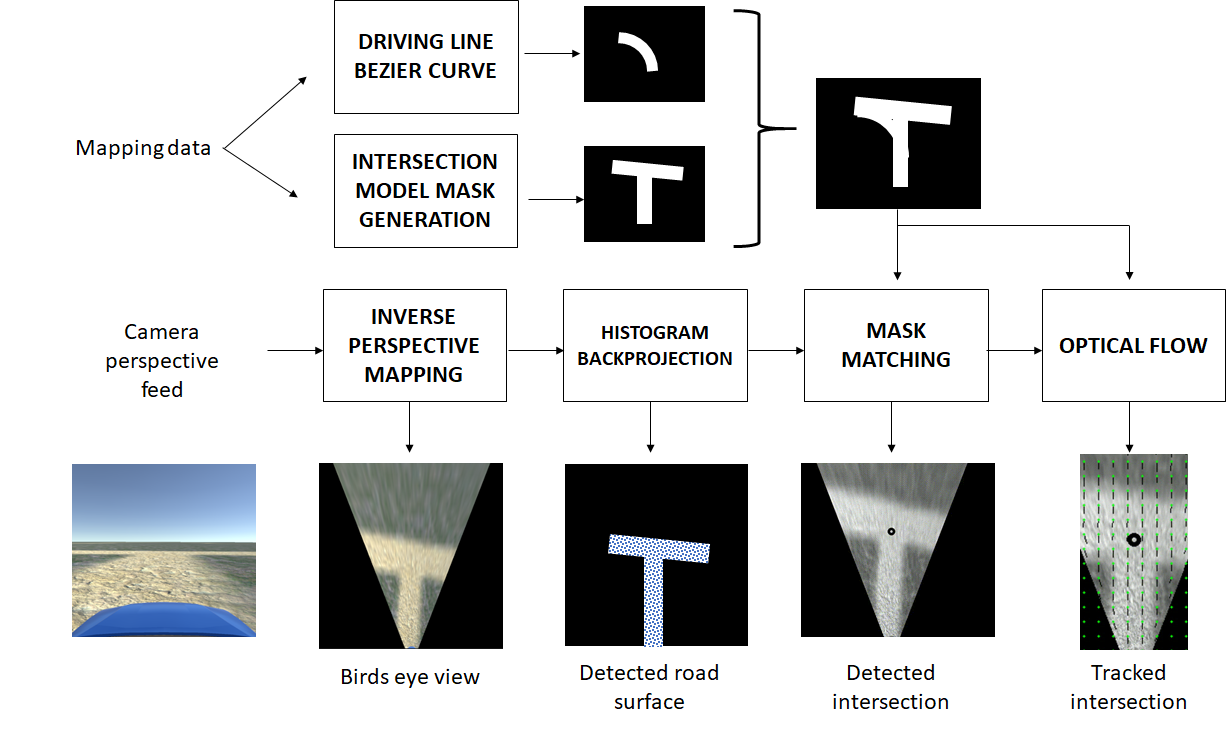
\includegraphics[width=0.95\textwidth]{systemOverview.png}
	\caption{High level overview of system stages, inputs and outputs.}
	\label{f:systemOverview}
\end{figure}


In general, the system uses inverse perspective mapping to develop a `top down' projection from the front facing vehicle camera image. \textbf{TODO: Refer to the appropriate figure for each of these steps}. An averaged histogram of local road pixels is used to develop a probabilistic road surface map using histogram backprojection. The system uses route `features' to localise the navigation goal. Route features used in the development of the system were road intersections\footnote{Examples in this paper generally consider an approach to a T junction in a custom built simulation.} however any point on a route with a clear visual pattern for the approach and exit(s) can be used. Route features are developed from mapping data (such as Open Street Map or Google Maps data) using road position nodes. A binary image mask of the upcoming route feature is developed using mapping data and is overlaid on the detected road surface. The feature is deemed detected when the proportion of feature mask covered by road surface is above a threshold. Once initially detected, the feature position is updated in subsequent video frames using a mean optical flow between frames and confirmed by remasking. A driving line through the feature can be developed and tracked by using a Bezier curve of the desired route through the feature once the initial feature model has been detected.

The discrete elements of the system with input and output as follows: 

\begin{easylist}[itemize]
	& \textbf{Road surface detection}. 
	&& \textbf{Input: }Camera feed.  \textbf{TODO: Defined data representations (F frames per second, nxm pixels x 32 bits)}
	&& \textbf{Output: }`top down' road surface map. 

	& \textbf{Route feature matching}. 
	&& \textbf{Input:} `top down' road surface map. 
	&& \textbf{Input:} Route feature generated from mapping information. 
	&& \textbf{Output: }Position in image of target route feature, if detected.
%	&& Route model mask matching
%	&& 
%	
%	&& \textbf{TODO? Explain - Inverse perspective mapping and camera lens distortion correction}
%	& Probabilistic road surface detection
%	&& \textbf{TODO? Explain - Rolling average histogram for road surface estimation}
%	& Local orientation to road edges
%	&& \textbf{TODO? Explain - Hough transform (IS THIS NEEDED?)}
%	& Route feature matching
%	&& \textbf{TODO? Explain - Matching piecewise model to detected road surface by masking}
%	& Optical flow tracking
%	&& \textbf{TODO? Explain - Using image `flow' to track feature positions for subsequent frame matching and cornering}
%	& Driving path curve matching
%	&& \textbf{TODO? Explain - Bezier curves based off feature points}
	& \textbf{Route feature tracking}. 
	&& \textbf{Input: } Previous image frame and detected location of target route feature for that frame. 
	&& \textbf{Output: }Updated location of target route feature in subsequent image frame.
\end{easylist}


\section{Related works}

Current cutting edge self driving vehicles require high fidelity 3D maps to operate effectively which are time consuming to develop and not adaptive to rapid local changes. Despite this, position localisation improvements have been achieved without high fidelity 3D mapping data using a data fusion of GPS and inertial navigation system data \citep{gpsInsFusion} correlating a detected back lane registry supported with computer vision, GPS and inertial data with map data \citep{lowCostSensorNav} and through use of Kalman filters and LIDAR in more complex environments \citep{robotLIDARSLAM}.


\citet{ipmBasedLaneDetectionApproach} also used inverse perspective mapping with k-means clustering and open uniform B-spline model for lane fitting. \citet{ipmForLaneTracking} outlined the effectiveness of Inverse Perspective Mapping for lane detection and \citet{canneyAndHoughLanes} outlined a robust lane detection approach using Canny edge detection and the Hough transform. \citet{ipmOpticalFlow} highlighted the effectiveness of inverse perspective mapping for optical flow computation, a finding that is strongly supported by the optical flow results obtained in this system.


Histogram backprojection has been used for basic \citep{histBackObjectTracking} and multi model object tracking \citep{histBackMultiObjectTrack}, \citep{histBackObjectMultiLighting}, image indexing \citep{histBackImageIndexing} and region of interest detection \citep{histBackObjectOfInterestDetection}. It has been used with sensor fusion including thermal mapping for road detection \citep{histBackThermal} and to effectively refine spatial fuzzy clustering road detection \citep{histBackRefineShadows}.

\citet{moncularLaneDetectAndTrack} outlined an approach involving the use of a Support Vector Machine to segment image road pixels from non-road pixels and an identification of road edges and control points defining the road curve. This approach is somewhat less interpretable however provides a suitable alternate and possibly more robust option for road detection. Additionally the input and output interfaces are the same as in this system which allows the option to `sub in' this approach if it is preferred. 

\citet{histogramSegmentationRoadClassification} investigated road classification from histogram based segmentation. Other road detection approaches include road surface mapping from near field driving surface models \citep{darpaChallengeRoadDetection} and matching road curvature models to detected lane boundaries \citep{intersectionDetectionSingleCamera}. Supervised convolutional neural network lane detection has had success through fully convolutional \citep{cnnLanes1} and instance segmented \citep{cnnLanes2} approaches. Spline based representation using random sample consensus for bezier splines based off road edge detection \citep{ransicBezierFit} has also shown to be effective.

\citet{modelBasedIntersection} outlined a model based recognition approached which matches intersection models to a series of road boundary points and \citet{mitLocalNavDriving} demonstrated through practical experiments that effective localisation using Open Street Map data and global waypoints is possible using a LIDAR sensor suite for local trajectory generation.




\section{Road Surface Detection}\label{s:roadSurfaceDetection}

In order to localise navigation elements a reasonable estimate of the current road surface is required. This is achieved via Inverse Perspective Mapping (IPM) and histogram backprojection. These aspects are discussed in detail in the following subsections. The road surface detection implemented is a basic road surface detection algorithm and can be outperformed by other more advanced methods. While it was suitable for developing the proof of concept system, more robust alternatives would be suggested in a live system.

\subsection{Inverse Perspective Mapping}\label{s:ipm}

\begin{figure}
	\centering
	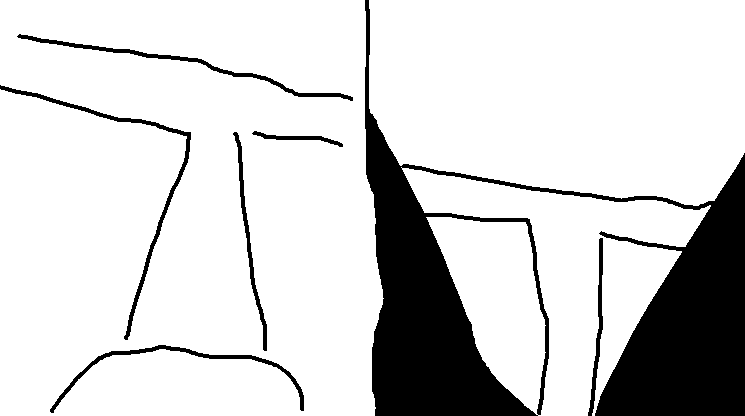
\includegraphics[width=0.95\textwidth]{RoadDetection/ipmSim.png}
	\caption{Example image from simulation (left) with IPM applied (centre) and derived IPM mask (right).}
	\label{f:ipmSim}
\end{figure}

Inverse perspective mapping (IPM) is a well established technique that involves a matrix transformation operation to remap pixels from a forward facing camera perspective to a `top down' view \citep{compVisionTextbook}. As part of this process the pixel to real world distance ratio of the inverse transformed image is determined based on known distances in the transformed image. An example of the technique applied to an image from the simulation used is included as figure \ref{f:ipmSim}. IPM assumes the perspective image is from a flat plane \citep{ipmForLaneTracking} and while road surfaces are not a flat plane, in most circumstances the local road plane can be considered approximately linear about a vehicle position as the scale of large road undulations do not generally result in significant changes locally to a vehicle. Further the system developed is robust enough to tolerate introduced error by \textbf{reasonable undulation - TODO: define (+/- x percent?)}. \citet{extendedIPM} have discussed an IPM approach that removes the flat plane assumption however it relies on a stereo camera so is out of scope for this system. This approach may prove more resilient and is worth consideration in the event a purely stereo camera based system is being developed. \textbf{TODO: Opportunity `blend' data from previous frames to estimate area outside IPM mask.}


It can be noted that the inverse perspective mapped image has a `null' area in the bottom edges where all pixels are black due to the perspective shift. This represents areas of the original perspective image that are outside the camera lens field of view. An `IPM mask' is developed which is used in later stages to ensure that any feature matching attempts are not penalised by the zero values in this area. The derived IPM mask is also included in figure \ref{f:ipmSim}. This is discussed again in section \ref{sect:route_feature_matching}. In order to correct for camera perspective as fully as possible, the camera lens effect should be corrected for \citep{fisheyeEffect} however the effects were negligible in this case and the system is robust enough that there was no requirement for this step.

\subsection{Probabilistic road surface detection}\label{s:histogramRoadDetection}

\begin{figure}
	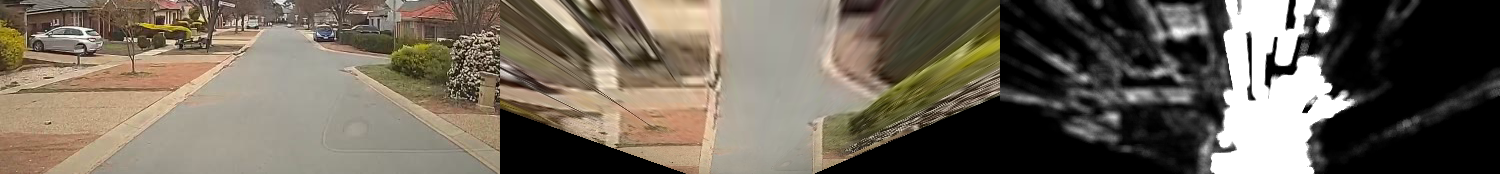
\includegraphics[width=0.99\textwidth]{RoadDetection/histRoadLive.png}
	\caption{Detected road surface from inverse perspective mapped live camera.}
	\label{f:histRoadLive}
\end{figure}

The road surface detection module uses histogram backprojection to identify likely areas of road surface. Histogram backprojection takes a provided histogram of the target, in this case the road surface, and divides it by an image histogram before convolution with a small mask to gain an estimation for the probability for each pixel in the image belonging to the target histogram \citep{histBackImageIndexing}. For this system, initially a road surface area of interest is defined, based off the near portion of road surface from the vehicle front, as indicated in figure \ref{f:histIPMcompare}. While this relies on the assumption that the vehicle starts on a road surface, it has the benefit of flexibility in detecting dynamic road surfaces. A histogram of this area is used to inform a rolling average histogram which considers the previous five frames. This is histogram is backprojected over the image to obtain a road surface probability for each pixel. An example of the detected road surface from an IPM transformed live camera feed is included as figure \ref{f:histRoadLive}. \textbf{TODO: Camera data}



While the road detection approach used for this system works with both the inverse perspective mapped image and the raw camera perspective image, in this instance it was applied after IPM transformation. It was clear from early tests that a better road surface detection was obtained when the IPM transformation occurred as the initial step \textbf{TODO: Quantify (refer to results)}. Figure \ref{f:histIPMcompare} demonstrates the significant degradation in detected surface quality when IPM transformation is applied after the road surface detection. It was also noted that when IPM was applied after road surface detection, probabilities were skewed based off pixel stretching as a result of the IPM transformation. For this reason it was determined that road surface detection should occur after IPM transformation.

\begin{figure}
	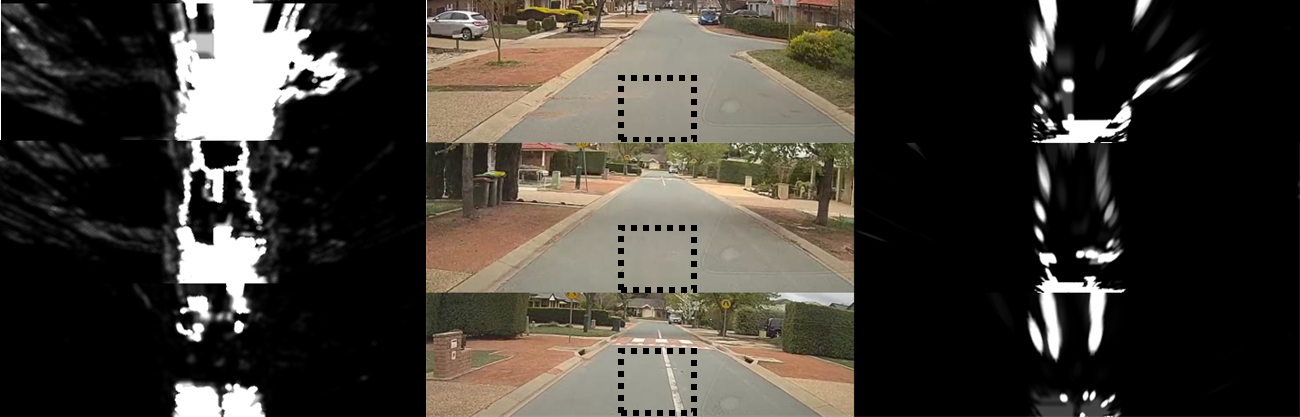
\includegraphics[width=0.99\textwidth]{RoadDetection/histIPMcompare.png}
	\caption{Comparison of histogram backprojection conducted after IPM transformation (left) and prior to IPM transformation (right). Raw image used (centre) includes indicative sampling area of interest used.}
	\label{f:histIPMcompare}
\end{figure}



%\begin{wrapfigure}{h}{0.5\textwidth} %this figure will be at the right
%	\centering
%	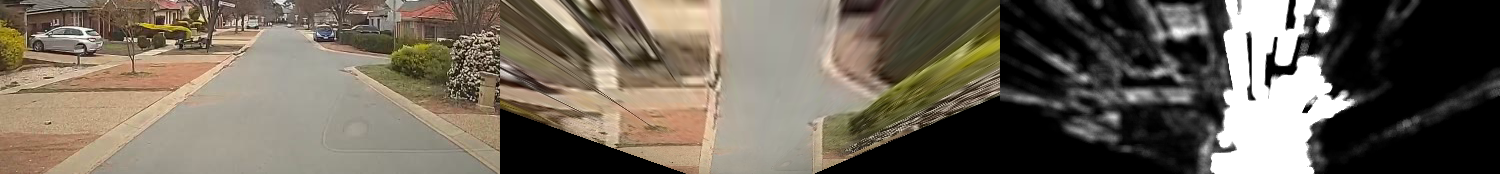
\includegraphics[width=0.5\textwidth]{RoadDetection/histRoadLive.png}
%	\caption{Detected road surface from live camera.}
%	\label{f:histRoadLive}
%\end{wrapfigure}


\citet{histBackRefineShadows} outline a shortfall with this style of road surface detection is that it can be prone to error when the road surface has little colour difference to the surrounding environment. The approach suggested in that case includes the use of thermal sensing so is not applicable for this system. If the system is required to operate in a more difficult to segment environment a more robust road detection approach may be needed. 


\section{Route Feature Matching}\label{sect:route_feature_matching}

\textbf{The system matches route `features' based on points defining relevant road segments - TODO: Expand on this for reader}. While GPS mapping data format can vary, the general common factor is that roads are defined by a series of points (nodes). These points can be used to develop a model of the road and in this case, key features. Features considered involved road intersections such as T junctions and side roads. The `main feature node' is considered to be the node central to the feature, for example the node in the middle of an intersection. A developed feature mask is used to determine if the detected road pixels match the feature. The following subsections outline the development of the route feature mask, the driving line mask and the subsequent matching process.

\subsection{Feature mask development} \label{s:maskDevelopment}

In order to develop a feature model, the feature point (node central to the intersection in this case) was placed as a starting point centrally on a blank mask. The feature mask is then developed by linearly connecting adjoining nodes. The pixel distance between nodes is defined based on the real world distance between nodes scaled using a pixel to real world distance ratio that is identified during the IPM process. It is important to note at this stage that the feature mask consists of multiple sub masks; each connection to the feature point is kept as an independent mask \footnote{Maintaining individual sub masks results in a more robust feature detection. This is discussed later in the paper.}. The width of these connections is scaled to the desired projected width for vehicle movement. An overview of the feature mask creation is included as figure \ref{f:featureMaskDevelopment} with the individual sub masks being represented by differing shading in the central sub figures. The final step in developing the feature mask is to mask it to the non-null areas of the inverse perspective mapped image. This is done using a bitwise AND operation between the developed feature mask and the IPM mask. The purpose of this step is to ensure that portions of mask features such as side roads are not considered if they fall outside the inverse projected image space. 

\begin{figure}
	\centering
	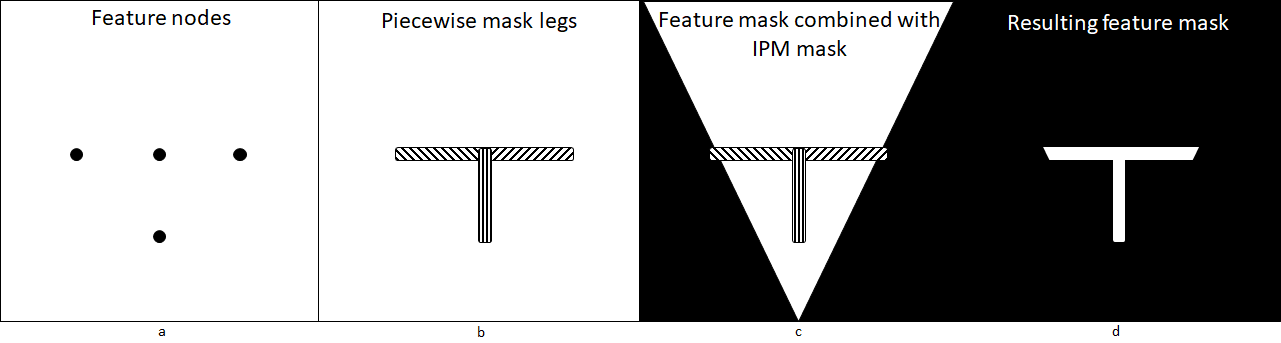
\includegraphics[width=1\textwidth]{FeatureMatching/featureMaskDevelopment.png}
	\caption{Process of developing feature mask developed feature nodes. Nodes are placed (left) and individually connected to main feature node (centre left). Shading differentiates between sub masks. The initial feature mask is then combined with the IPM mask (centre right) to obtain the final model mask (right)}
	\label{f:featureMaskDevelopment}
\end{figure}

For this system, the mask development process only considered the feature node and immediate connecting nodes. A more robust approach which considers additional approach nodes is discussed in section \ref{s:discussion}-\ref{s:improvements}.

\subsection{Driving line curve mask} \label{s:drivingPathMatching}

In order to allow a controller to effectively action system outputs there needs to be consideration given to vehicle turning arcs. This is addressed by incorporating a `driving line curve' into the mask to ensure the detected feature has room for the vehicle to turn through it. The driving line curve mask is developed using a quadratic bezier curve defined by the approach node, the feature node and the exit node. Once the driving path curve mask is developed it is masked by the IPM mask and added to the route feature masks in order to ensure the developed driving line is also on a detected road. 

The quadratic bezier is generated simply by a series of linear interpolations over the range $t=0...1$. Linearly interpolating \textit{t} between the approach node to feature node and the feature node to exit node provides two new points, \textit{p0} and \textit{p1}. Linearly interpolating \textit{t} between \textit{p0} and \textit{p1} provides a point \textbf{B(}\textit{t}\textbf{)} along the quadratic bezier curve. The full bezier curve is given by \textbf{B(}\textit{t}\textbf{)} for the range $t=0...1$. A visualisation of this is included as figure \ref{f:quadraticBezier}.

\begin{figure}
	\centering
	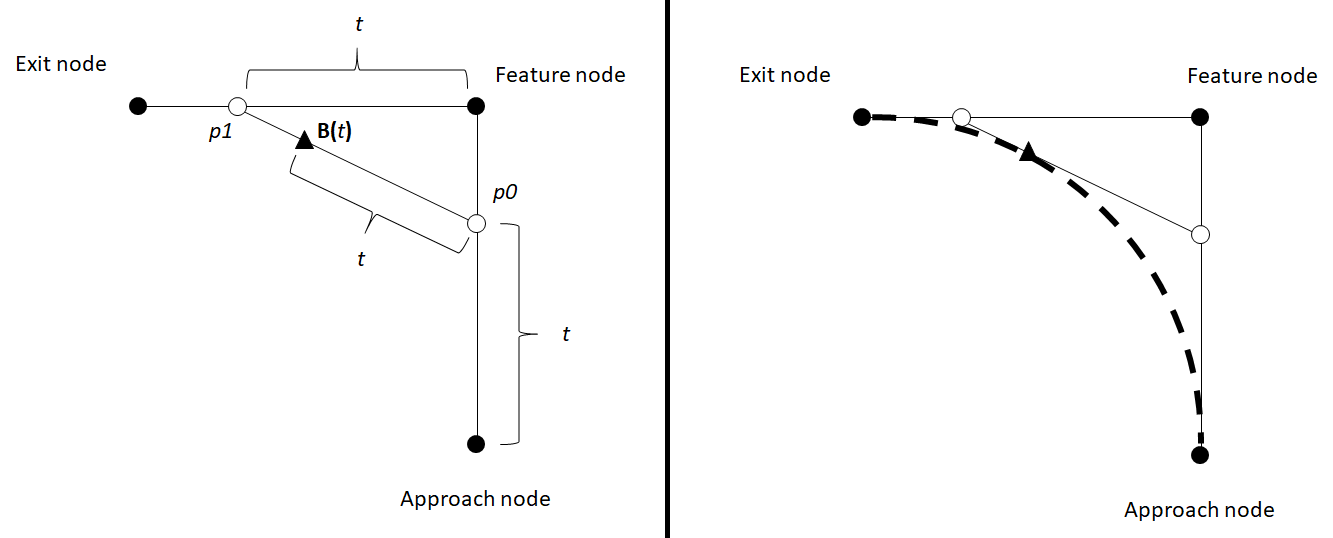
\includegraphics[width=1\textwidth]{bezier/quadraticBezier.png}
	\caption{Bezier curve interpolation: Generating \textbf{B(}\textit{t}\textbf{)} for $t\approx0.7$ (left) and the full bezier curve (right)}
	\label{f:quadraticBezier}
\end{figure}

The development of the driving line will generally need to be customised for the specific vehicle implementing this system in order to account for specific parameters such as turning circle. This is implemented by amending the approach and exit node to be a desired distance from the feature node such that a developed bezier curve represents the turning circle capability of the vehicle. 

\subsection{Feature mask matching} 

Features are considered detected based off a probability threshold; that is a feature is considered as a binary `detected' or `non-detected' based on a comparison between a defined threshold and the determined probability. Let $P(\textbf{F})$ be the probability that a feature $\textbf{F}$ is detected for a given detected road surface $\textbf{R}$ and $P(\textbf{F}_{sub,k})$ be the probability that the k'th sub feature $\textbf{F}_{sub,k}$ is detected. $P(\textbf{F}_{sub,k})$ is determined by the summation of the Hadamard product (elementwise product) between the feature sub mask and the detected road surface divided by the element sum of the feature sub mask, as outlined in equation \ref{eq:subMaskProbability}. The assessed probability that the route feature is detected is the minimum sub feature probability as per equation \ref{eq:featureProbability}. The probability threshold for $P(\textbf{F})$ is a design decision that can be amended based on factors such as noise and road surface detection output, for example considering a probabilistic or binary thresholded detected road mask. \textbf{Talk about what was explored as thresholds and consequences.}

\begin{equation}\label{eq:subMaskProbability}
	P(\textbf{F}_{sub,k}) = \frac{\sum_{i,j=1}^{n} (\textbf{R} \circ \textbf{F}_{sub,k})_{ij}}{\sum_{i,j=1}^{n} \textbf{F}_{sub,k,ij}}
\end{equation}

\begin{equation}\label{eq:featureProbability}
	P(\textbf{F}) = min\{\textbf{F}_{sub,k}:k=1,...,n\}
\end{equation}

Initial detection approaches involved using a single full feature mask as per equation \ref{eq:subMaskProbability} in lieu of sub features however this approach is significantly less robust. In the event of a noisy surface detection it is conceivable that the sum total of all road pixels under the mask may meet a generous threshold even if one element of the feature is not detected at all. Considering all elements of the feature as separate masks and using the minimum detected probability eliminates this and ensures that each feature element has a minimum detection. 

Once the feature is detected, the centre point is then the main feature node location from the initial mask. It is possible to further refine this by `bracketing' about the detected feature point by testing surrounding points. This may not be required however as assuming the vehicle is central on the road surface the midpoint of the detected feature will be aligned to the midpoint of the route feature and the inclusion of the driving line in the feature mask assures the chosen line is on the detected road surface.

\section{Route Feature Tracking}\label{s:roadFeatureTracking}

Mean optical flow was used to estimate an updated feature node location in order to track the detected route features. This was then confirmed using the masking approach discussed in section \ref{sect:route_feature_matching}. In general, optical flow options can be considered as sparse where a few key points are tracked, or dense where a large number of points up to individual pixels are tracked. It should be noted this categorisation represents ends of a continuous range rather than a binary category option. 

The Gunnar Farneb{\"a}ck method \citep{opticalFlowSolution} is a dense approach which considers a polynomial expansion to approximate pixel neighbourhood and minimises an error function for an approximated local displacement. By contrast, the Pyramidal Implementation of the Lucas Kanade Feature Tracker outlined by \citet{opticalFlowLKPyramidal} relies on key tracking points in an image. The Lucas Kanade approach was considered initially as a sparse option due to efficiency however it did not perform well. It is assessed that the random surface textures in this case lack the definition to be tracked effectively via this method. The Two Frame Estimation proposed by \citet{opticalFlowSolution} (the `Gunnar Farneb{\"a}ck method') was identified to perform better in the image frames that are typical of this problem. Similar relative performance results were identified by \citet{opticalFlowLKvsDenseUAV} when considering moving images of near grass surfaces. The Gunnar Farneb{\"a}ck method was employed to track pixels in a small region of interest on the inverse perspective mapped camera image. The region of interest is comparable to the histogram region of interest for backprojection as discussed in section \ref{s:roadSurfaceDetection}-\ref{s:histogramRoadDetection}. The smaller region of interest mitigated the use of a dense algorithm while improving mean optical flow calculation accuracy.

\begin{wrapfigure}{r}{0.35\textwidth} %this figure will be at the right
	\centering
	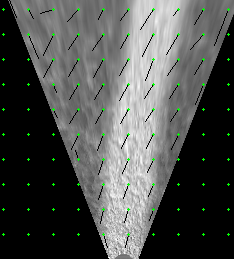
\includegraphics[width=0.35\textwidth]{FeatureTracking/optical_flow_trails.png}
	\caption{Selected optical flow lines visualised. Black tails indicate flow vector from each point.}
	\label{f:optical_flow_trails}
\end{wrapfigure}

The benefits of optical flow tracking in a smaller region of interest of the inverse perspective map are as follows:
\begin{easylist}
	& Allows effective processing of dense optical flow due to a small total number of pixels.
	& Avoids noisy areas such as extremity pixels which are warped by IPM.
	& Optical flow space occurs in the same space as the feature matching allowing a direct application of mean flow to the new estimated position.
\end{easylist}

A visual example of optical flow output for a small selection of pixels is included as figure \ref{f:optical_flow_trails}. It can be seen from this image that not all flow vectors are uniform and in particular at the edges of the mask there are large distortions. These distortions are expected due to the discontinuity and do not affect the result as the system only considers the optical flow from a range of pixels to the direct front of the vehicle. The average of these more uniform flow vectors is used to provide an effective estimate of the updated feature location. The mean optical flow approach involving a small region of interest of 100px high by 36px wide performed effectively in cases where the mean flow was in the order of 5px or less, corresponding to an approximate 5\% of the window height. \textbf{TODO: RESULTS FROM PRESENTATION.}

Once the mean optical flow has been developed, the estimated feature position is updated and the position delta is also used to update the feature model masks accordingly. Once the model masks have been updated, the IPM mask is applied and the new approximated feature position is confirmed using route feature matching as discussed in section \ref{sect:route_feature_matching}. If the new location of the approaching node places the curve defined by the driving path at the bottom of the image, the vehicle has arrived at the tracked feature and the route feature matching can generate the next route feature. In the event the feature is otherwise no longer detected, a bracketing approach can be used to attempt to relocate it.

\section{Discussion} \label{s:discussion}

\textbf{TODO: Start positively - This system as developed effectively identifies route features and driving lines through features. The system was developed and refined in simulation with verification conducted using live dashcam footage. }The system outlined in this paper does have the limitation that it is designed around a single road surface which is assumed to be fully drivable. Multi lane detection and detection and tracking of other vehicles is outside the scope of the system as developed. While a controller may manage these factors, there is no explicit consideration for non traversable road surfaces (for example a lane with opposite direction of travel) or on road obstacles. Within these specified limitations however, the system as outlined demonstrated an ability to approximate a road surface and very effectively identify and track route features and driving lines where the road surface identification was effective. The system is easy to understand at a high level, as per figure \ref{f:systemOverview} and has interpretable inputs and outputs which can be used in other aspects by both human and machine applications. This provides a system suitable for navigation localisation redundancy or alternatively in a low cost entry level setup.

\textbf{System parameters.} The system has a range of parameters to be specified which allow customisation to both vehicle and route specifications. System parameters include: 

\begin{easylist}
	& \textbf{Camera parameters.} \textbf{TODO: Expand this section for future work (appendix)}
	&& \textbf{Field of view.} The camera field of view affects the visibility of road surfaces off the direct line of travel at the close edges of the vehicle, especially after IPM is applied. If the field of view is too narrow, route features such as side streets may be lost prematurely. As such, a field of view with reasonable vision to the left and right of the driving surface in the near distance is required.	
	&& \textbf{Frame resolution.} This system remains effective at lower resolutions so the full resolution of the camera frame may not be required. While larger frames contain more detail in general the system can trade some resolution for computational time savings without significant losses. Frame resolutions used in testing varied from 512px to 150px widths. 
	&& \textbf{Frame processing frequency.} While not strictly a camera parameter, the frequency with which the system processes the frames is a key consideration and will generally relate to the processing speed of the implementation. A lower frequency of frame processing results in a higher likelihood of route feature tracking errors and less redundancy in any detection failures. Frame frequency for this test was as low as 10Hz with no noticeable degradation in feature detection or optical flow tracking. This parameter should be considered in context with resolution to ensure that optical flow tracking remains effective.
	& \textbf{Road surface detection.}
	&& \textbf{Assumed road surface region.} The histogram backprojection relies on a specifieds area in front of the vehicle to be sampled for the histogram for backprojection. This region will vary based on the physical setup of the vehicle and camera mount and should be chosen carefully to avoid introduction of additional noise such as road edges. The size of this region is dependant on the camera field of view; a narrow camera field of view will restrict the area that can be reliably sampled as road surface.
	&& \textbf{Feature detection probability threshold.} This value is considered when determining if a feature has been detected. A value of 1.0 will require each pixel of the feature mask to be over a road surface pixel with a probability of 1.0. The only occasion this is feasible is in the case the detected road surface is a purely binary thresholded mask. Realistically the detection threshold probability needs to be less than 1.0 to account for noise and uncertainty in the detected road surface.
	& \textbf{Feature development}
	&& \textbf{Image pixel to real world distance ratio.} This can be determined from the IPM procedure based on known real world distances as projected after IPM occurs. This is required for the development of route feature masks at an accurate scale. 
	&& \textbf{Route feature mask width.} The pixel width to use when developing the route feature mask. This width does not need to represent a full vehicle width as the driving line mask will ensure the vehicle can pass through the feature. In the development of this system, the route feature mask width was 25\% of the vehicle width. If this width is too great there is a risk that the combined driving line and feature mask may be wider than the feature itself, leading to a failure to detect the feature.
	&& \textbf{Driving line mask width.} Related to above however this needs to have a real world width to comfortably accommodate the vehicle width to ensure driving line through the feature will ensure the vehicle remains on the detected road surface.
\end{easylist}

These parameters directly impact the effectiveness of the system however are generally easy to tune as the entire system is human interpretable thus the effect of a parameter can be directly observed and understood.

\textbf{IPM and optical flow effectivenes.} \textbf{TODO: Does this need to be chopped? Integrated into results? other?} As noted in section \ref{s:roadSurfaceDetection}-\ref{s:ipm}, IPM transformation has the assumption of a flat plane which will not be the case along many routes. It was assessed that the local area in front of the vehicle \textbf{can be assumed to be linearised and testing demonstrated negligible affect on the localisation system TODO: why can it be assmued (+/- range) and what is the negligable affect? Quantify and refer to results? }when route undulations were incorporated. As a result it is assessed that this assumption can be held as feasible in standard driving conditions. It should also be noted that the optical flow estimation of the updated feature position was very effective in testing and once detected, features were not lost until arrival at the feature location. Regardless, as discussed in section \ref{s:roadFeatureTracking} it is important to build in redundancy and any controller implementing this system will need to include suitable actions in the event of complete feature loss.

\subsection{Performance}

It is somewhat difficult to effectively quantify the performance of the system as a whole as there is no relevant system benchmark and the `detection' module is deterministic in the sense that if the road surface is identified sufficiently, the feature mask matching process will identify the feature. Despite these factors it is important to quantify the performance of the system. The two core critical elements of the system are the road surface detection and the feature tracking. These elements are discussed in detail in following subsections.

In general the system has a computational complexity of \textbf{O(mn)} where the image frames are of dimension $m\times n$. The complexity directly scales based on input image dimensions which can be an initial simple parameter to consider for performance. The system was developed using simulated $512px \times 512px$ images and was validated with live video which was tested at a lower resolution of $400px \times 174px$.

It should be noted that many of the module operations as outlined are trivially parallisable. Specific implementations will require individual optimisation to identify the optimal operating parameters based on hardware available and road surface complexity. The test computer used had a 2013 model i5-3570k CPU. With the base implementation code implemented in Python, OpenCV and Numpy (with no optimisations), the system took on average\footnote{Multiple tests were benchmarked for time during final testing. Exact frame count was not obtained but consisted of data from at least 15000 frames of feature detection and 5000 frames of feature tracking.} 13.8769ms to process a single frame ($512px \times 512px$) in the Feature Matching state and processed individual frames in an average of 72.0621ms when tracking features with a region of interest of ($260px \times 55px$) using a three level Gunnar Farneb{\"a}ck detection.

\subsubsection{IPM and Histogram Backprojection}

While the IPM and Road Surface Detection modules have been discussed individually, it was identified that the accuracy of the detected road surface was dependant on the IPM implementation. When defining the IPM transformation initially, the `far' distance of the IPM transformed image is defined by the choice of pixel locations to transform (and their transformed locations). Tests were done using live image data with IPM transformation maximum projection distances consisting of far (100m), mid (30m) and near (15m). Indicative examples of the results of these distances for straight and curved roads is included as figure \ref{f:ipmHistogramResults}.


\begin{figure}{}
	\centering
	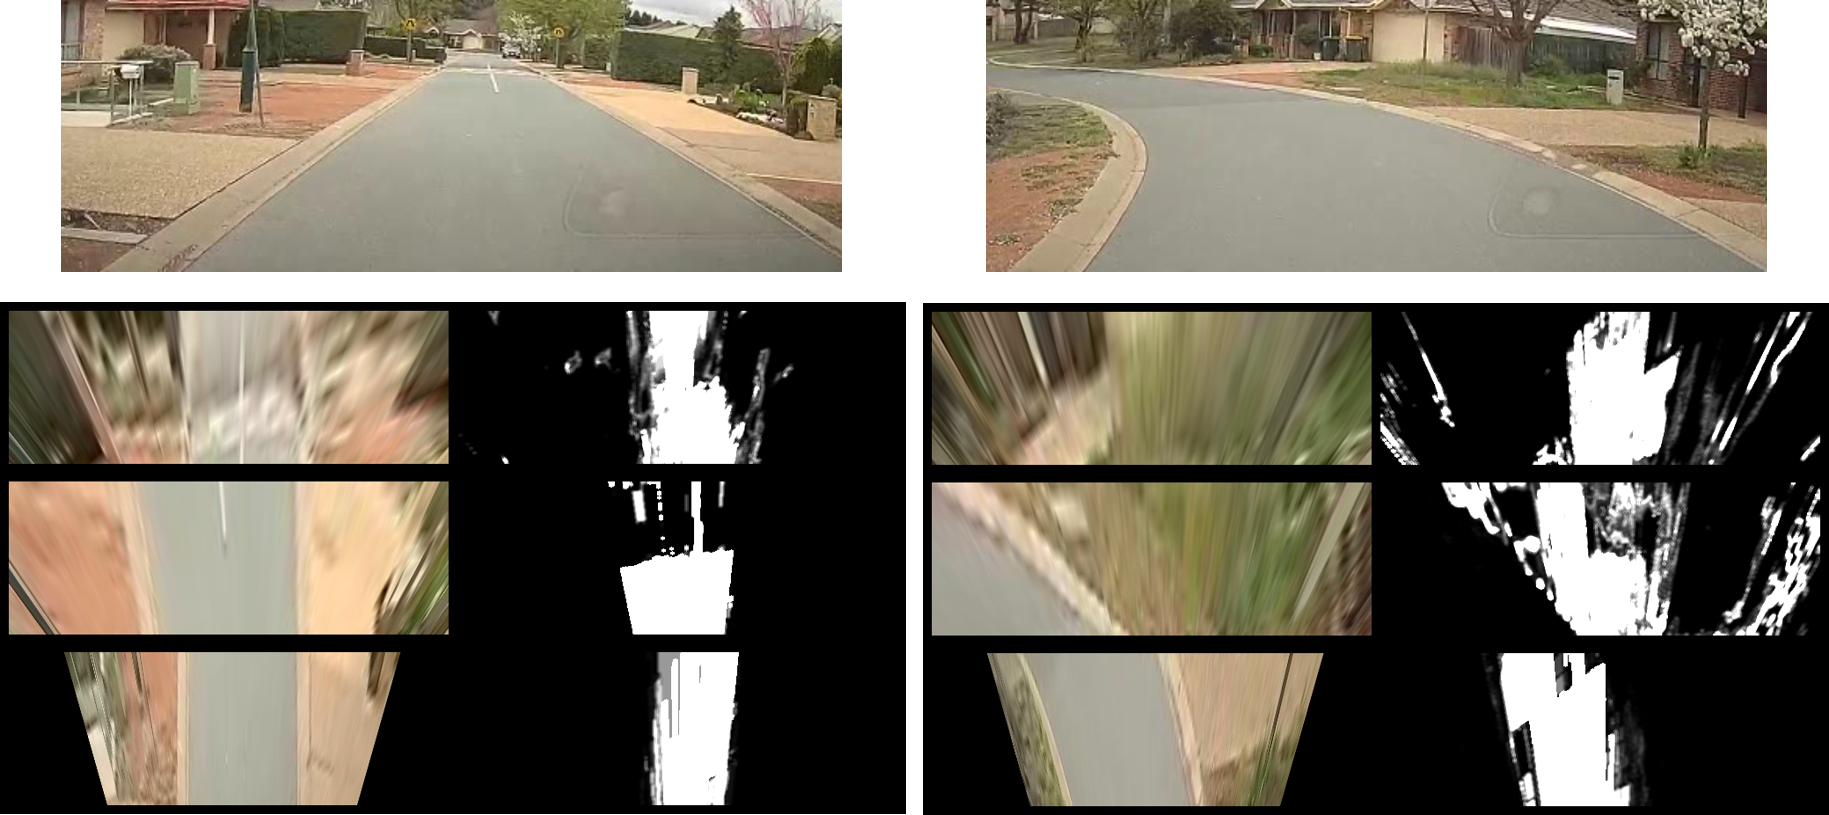
\includegraphics[width=0.99\textwidth]{Results/ipmHistogramResults.png}
	\caption{Demonstration of Histogram backprojection at far (top), mid and near (bottom) ranges for straight (left) and curved (right) road surfaces.}
	\label{f:ipmHistogramResults}
\end{figure}

An analysis of the road surface detection accuracy demonstrates that the near IPM range performs more consistently and, importantly, suffers from less `false positives' where road surface is detected outside the true surface. Table \ref{t:ipmRangeRoadSurface} outlines the accuracy values in these cases where it can be noted that the near maximum distances detects in the order of 75\% of the road surface consistently. 


\begin{table}[]
	\centering
	\begin{tabular}{@{}cccc@{}}
		\toprule
		Road type & IPM range & Correct road surface ratio & Falsely detected road surface ratio \\ \midrule
		Straight  & Far       & 67.186\%                   & 1.148\%                             \\
		& Mid       & 43.761\%                   & 0.391\%                             \\
		& Near      & 74.868\%                   & 0.486\%                             \\
		Curved    & Far       & 0\%                        & 20.558\%                            \\
		& Mid       & 0\%                        & 30.798\%                            \\
		& Near      & 75.261\%                   & 0.818\%                             \\ \bottomrule
	\end{tabular}
	\caption{Accuracy of detected road surface for varying IPM maximum ranges for straight and curved roads}
	\label{t:ipmRangeRoadSurface}
\end{table}

Road surface detection was also applied prior to IPM transformation as part of the validation process. Testing over multiple road \textbf{TODO: types? curves? straight etc} identifed that the quality of detected road surface degraded by as much as 50\% if detection was applied prior to IPM transformation. Figure \ref{f:ipmHistorgramReverse} demonstrates the result of applying road surface detection to the perspective image and applying the IPM transformation to the detected road surface. This detection example corresponds to the `near' range detection in figure \ref{f:ipmHistogramResults} and clearly demonstrates additional distortion to the IPM transformed road surface and the benefits of applying the IPM transformation prior to road surface detection.


\begin{figure}{h}
	\centering
	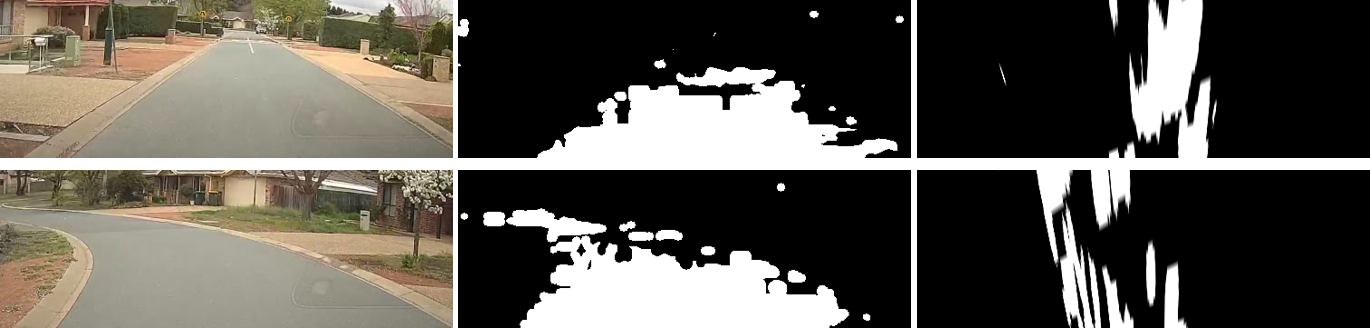
\includegraphics[width=0.99\textwidth]{Results/ipmHistorgramReverse.png}
	\caption{Road surface detection performance when applied prior to IPM transformation for roads in figure \ref{f:ipmHistogramResults}.}
	\label{f:ipmHistorgramReverse}
\end{figure}

%
%\begin{wrapfigure}{r}{0.95\textwidth} %this figure will be at the right
%	\centering
%	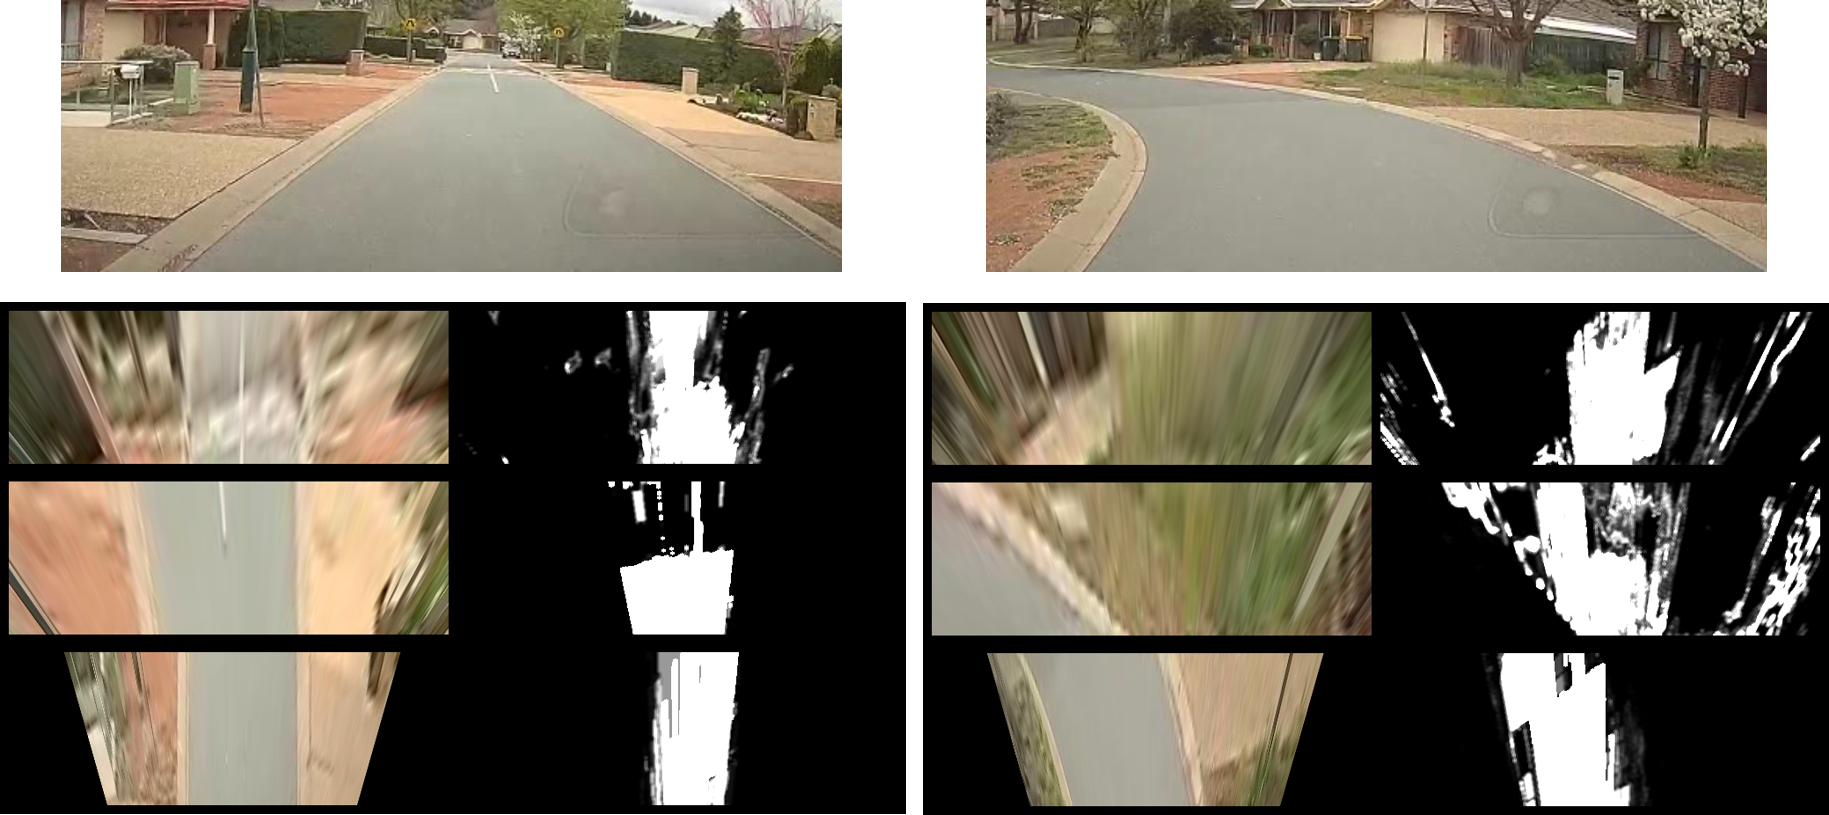
\includegraphics[width=0.95\textwidth]{Results/ipmHistogramResults.png}
%	\caption{Selected optical flow lines visualised. Black tails indicate flow vector from each point.}
%	\label{f:ipmHistogramResults}
%\end{wrapfigure}


\subsubsection{Optical Flow reliability}

The optical flow reliability is the second core element of the system that can be quantitatively investigated. The performance of this module was determined to be a combined function of image resolution and processing frequency. Optical flow error or `slippage' was defined as the apparent slipping of the detected feature; this was due to the computed mean optical flow being less than the true optical flow which resulted in the feature location not being moved the full delta each frame. It was determined that the resolution of the `area of interest' used for optical flow calculation was an effective comparison point and, as highlighted in figure \ref{f:opticalFlowResults}, the `slippage' has a generally linear relationship with increasing relative pixel flow.

\begin{wrapfigure}{r}{0.5\textwidth} %this figure will be at the right
	\centering
	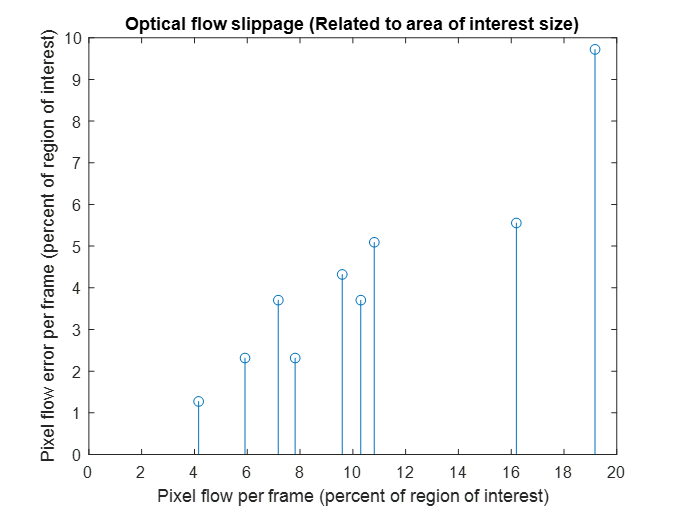
\includegraphics[width=0.5\textwidth]{Results/opticalFlowResults.png}
	\caption{Selected optical flow lines visualised. Black tails indicate flow vector from each point.}
	\label{f:opticalFlowResults}
\end{wrapfigure}

Increasing the resolution of the optical flow area of interest or increasing the processing frequency will result in a smaller relative pixel flow per frame which in turn will reduce the feature tracking error.

\subsection{Opportunities for future work} \label{s:improvements}

\textbf{TODO: Improved road surface detection (eg. CNN?)}

\textbf{Integration with Fuzzy Logic.} \citet{fuzzySail} present results demonstrating a very effective combination fuzzy control system for a sailing boat including the ability to tack and jibe. \citet{fuzzyGrove} outlined significant improvements in using fuzzy logic for sensor fusion and control of autonomous vehicles operating in citrus grove alleys. The system discussed in this paper involves probability based decisions throughout the process and may be a good candidate for integration with Fuzzy logic decision making and/or control.

\textbf{Known road map histograms.} The histogram backprojection uses an average histogram over the previous 5 frames. This is effective for slowly changing road surfaces however can lead to brief road surface loss when moving from one surface to another. An alternate option is to have a bank of representative road surfaces to use for the backprojection and consider the maximum probability over the range of surfaces as each pixel's probability of being a road surface. This can also be combined with the rolling average to provide a more robust assessment as well as categorise road surfaces. \textbf{TODO: Lighting effects - shade, time of day.}


\section{Implementation discussion}
\textit{\textbf{During the course of development of the single camera autonomous vehicle navigation localisation system, several implementation points were identified. These points were deemed outside the scope of discussion in the original article however are included here in an effort to preserve the information. This information is of particular importance to those interested in implementing or extending the system.}} \textbf{TODO: Reword this for journal article}



\subsection{Road surface centreline detection}

While vehicle position and orientation on the road is a critical input to a controller, it was not explicitly covered as part of this system. A general approach slightly modified from that outlined by \citet{canneyAndHoughLanes} to suit this system is to identify the central point on a road surface is to apply edge detection to the detected road surface pixels followed by identifying straight line candidates using the Hough transform. The basic approach would be as follows: 

\begin{easylist}
	& Identify local window of interest in the near ground to vehicle.
	& Use edge detection such as the Canny algorithm to identify road edge pixels inside window of interest.
	& Identify candidate lines using Hough Transform.
	& Select strongest candidate lines for left and right portions of the window, corresponding to the estimated left and right road edge lines.
	& Identify road centreline as midline between left and right detected edge lines.
	& Determine desired steering direction based on detected centreline pixel offset from vehicle centreline \footnote{The vehicle centreline will correspond to the image centre assuming the camera is position centrally. If the vehicle mounted camera is offset, this `centre pixel line' will need to be manually identified and stored prior to operation.}
\end{easylist}

This approach can be applied to either the camera perspective image or the IPM transformed image. In the former case the perspective effect where the left road edge line will be angled to the right and vice versa for right edges, tending to the vanishing point, allows easy segregation of left and right road surface lines. By contrast the IPM transformed road edges will be parallel thus rely on positional information only to separate the left and right road surface lines. Alternatively more advanced methods such as the Support Vector Machine approach suggested by \citet{moncularLaneDetectAndTrack} may be more robust and may additionally inform the road surface detection.



\textbf{Extension of feature masks.} As designed, the current system only considers the main feature node and immediate connections. As the feature node is placed centrally, the approach node distance results in only masking a small portion of the full image. An improvement is to extend the sub masks from the feature node to the full extent of the mask image size. This would involve each sub mask drawing additional relevant node connections until the relative position takes the line off the edge of the image. The resulting mask will be a full representation of the approach route to the feature.

\begin{wrapfigure}{r}{0.35\textwidth} %this figure will be at the right
	\centering
	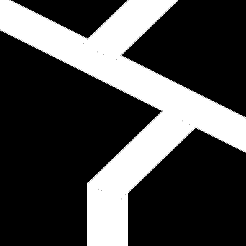
\includegraphics[width=0.35\textwidth]{complexFeatureApproach.png}
	\caption{An example of a complex approach to a feature which may undermine the current system feature detection.}
	\label{f:complexFeatureApproach}
\end{wrapfigure}

\subsection{Rotation of feature masks.} The current implementation has the system generating feature masks of the route feature as it will be approached and assumes a linear approach. This is a reasonable assumption for close in detection however it may fall down if complex approaches to route features are encountered. A more robust solution would involve developing the extended feature mask as outlined above and aligning the mask to the approach direction at the frame the feature will be detected. This would entail developing the mask as per section \ref{sect:route_feature_matching}-\ref{s:maskDevelopment} in the original paper and once developed, the mask can then be rotated so the approach line is vertical at the base of the image. On arrival at a feature node on the approach, the mask will be regenerated and reoriented. This approach takes advantage of the fact that the route between two nodes can be assumed as linear and will ensure the feature mask orientation will match the detected road more closely. 

An example of a complex approach to a feature is included as figure \ref{f:complexFeatureApproach}. In this instance as the vehicle encounters the first bend, the feature model mask will no longer have the correct orientation and result in a loss of feature tracking. 


\subsection{Navigation extension options.} While it was not explicitly considered as a feature, any road feature with a sharp enough angle between points can be used as a feature. This is particularly helpful if an aim is to identify a `true' position outside GPS error as bends in a road can be used as additional features without requiring additional intersecting roads. Additionally while this system was designed with a supporting GPS in mind to estimate anticipated feature arrival, as developed it does not rely on positional information specifically. Indeed assuming that relevant route feature data is stored, this system can work `offline' using the features as directions in a similar way a human navigator may. Integrating the output of this system with other sensors such as GPS offers additional localisation benefits. \citet{probabalisticRobotics} discuss Markov and extended Kalman filter localisation techniques that may be applicable to this system and have the potential to result in improved positional estimation.


\subsection{TODO}
Discuss Road detection mitigation (rolling average etc)
Add in references


\section{Concluding remarks}

\textbf{TODO: Start positively - This system does blah effectively and provides zzzz cabaility. }The resulting system has specified limitations as discussed in section \ref{sect:intro} and in particular the road surface detection approach represents a basic implementation. In addition to the societal considerations for interpretable AI, the focus on interpretable steps has the significant benefit of having a clear `plug and play' interface with other systems. As a result, when an improved road surface detection algorithm is identified it can easily be integrated to the system in place of the existing element. 

As developed, the system effectively identifies and tracks route features and provides a driving line through the identified feature. The model mask approach of feature detection provided effective feature matching in non ideal conditions and the bezier curve driving line provides a control system a constant steering angle for feature traversal. In particular the use of optical flow for route feature tracking was highly effective. 

Redundancy in autonomous systems is a critical consideration and should be included as part of any system design. A system such as the one proposed in this paper provides a low barrier to entry for simple vehicular navigation automation tasks and offers a final redundancy option in the event that a `high end' autonomous system suffers a significant sensor suite failure.

\textbf{TODO:}
The system was developed using simulated $512px \times 512px$ images and ran at over 70Hz while in the Feature Matching state, maintaining over 10Hz while feature tracking. The system was validated with live video which was tested at a lower resolution of $400px \times 174px$.

%\section*{Appendices}
%\ref{app:implementationDiscussion} - Implementation Discussion \\

\newpage

\bibliography{References}

%\appendix
%\pagestyle{empty}
%
%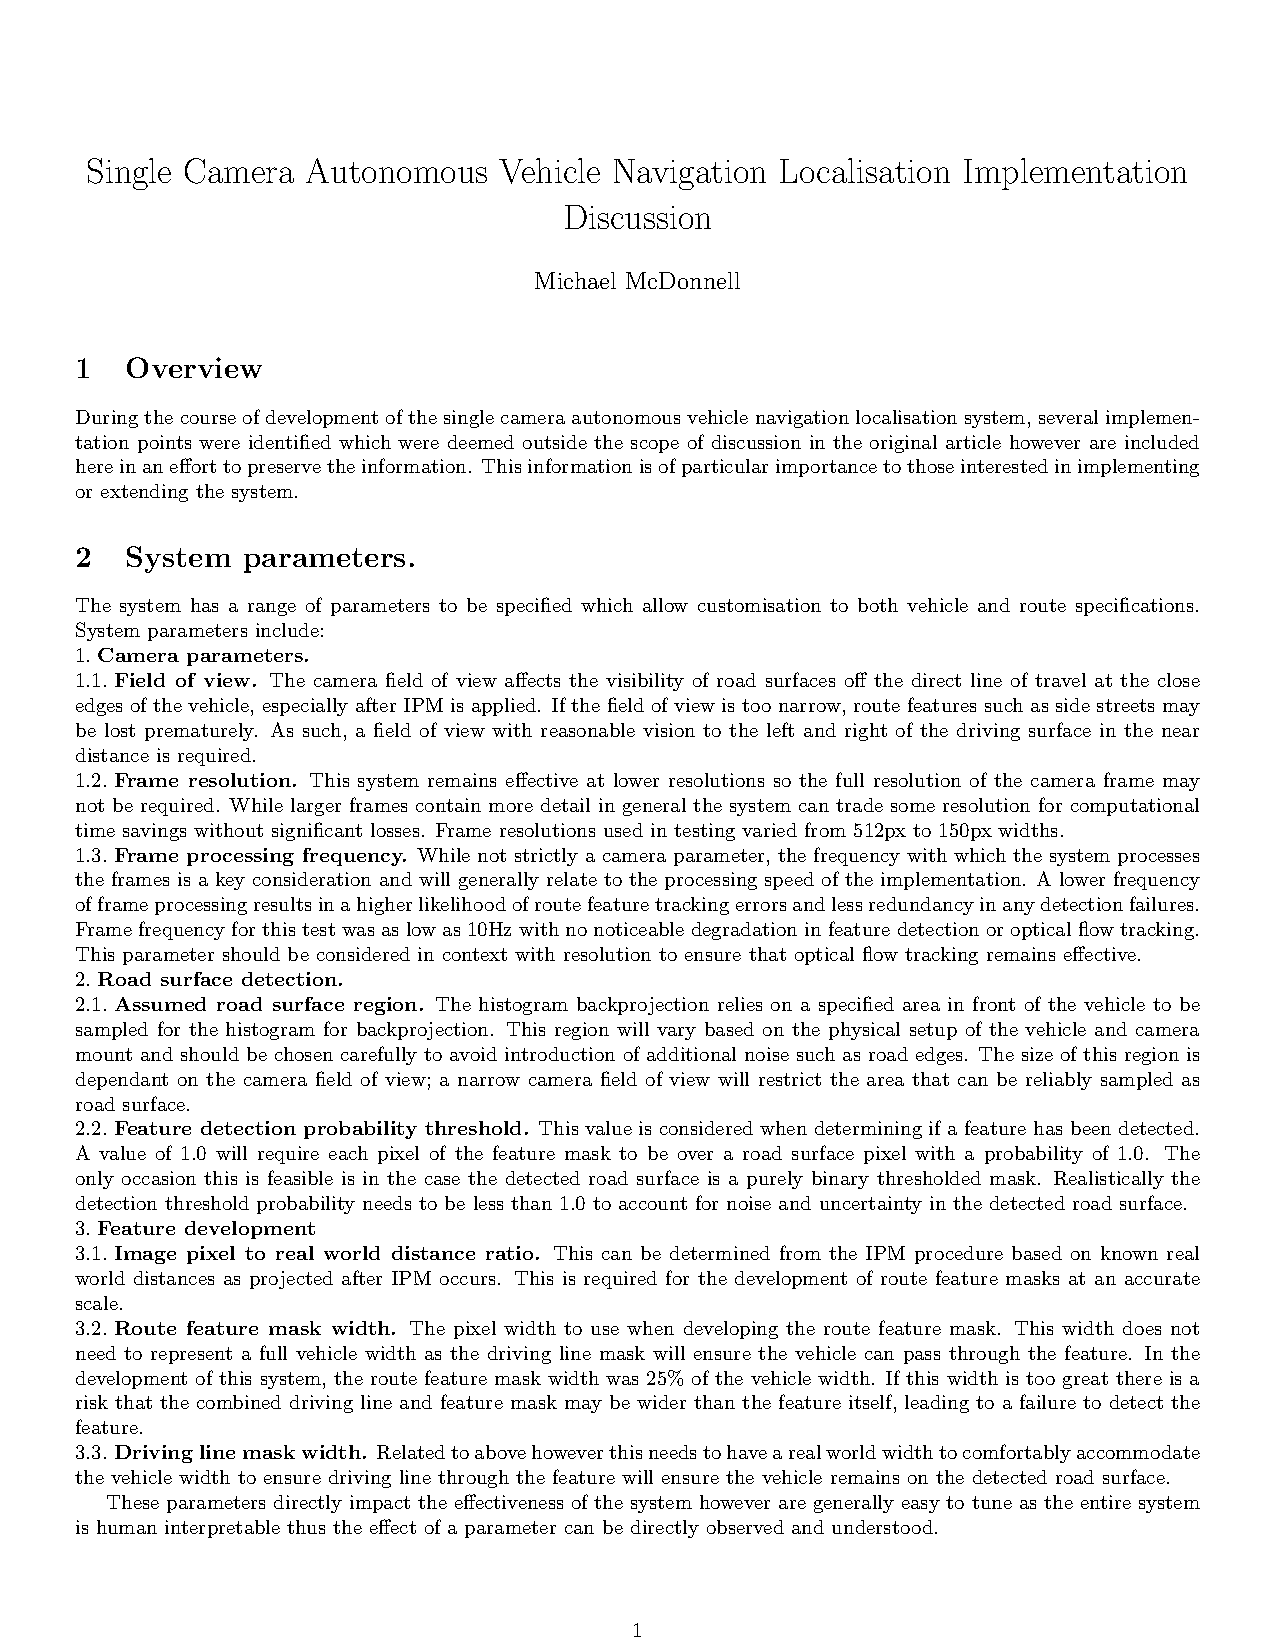
\includepdf[pages=1,scale=.9,pagecommand={\section{Implementation Discussion}\label{app:implementationDiscussion}},linktodoc=false]{implementationDiscussion.pdf}
%\includepdf[pages=2-,scale=.9,pagecommand={},linktodoc=false]{implementationDiscussion.pdf}




\end{document}

